%File: formatting-instruction.tex
\documentclass[letterpaper]{article}
\usepackage{aaai}
\usepackage{times}
\usepackage{helvet}
\usepackage{courier}
\usepackage{graphicx}
\frenchspacing
\setlength{\pdfpagewidth}{8.5in}
\setlength{\pdfpageheight}{11in}
\pdfinfo{
/Title (Insert Your Title Here)
/Author (Put All Your Authors Here, Separated by Commas)}
\setcounter{secnumdepth}{0}  
 \begin{document}
% The file aaai.sty is the style file for AAAI Press 
% proceedings, working notes, and technical reports.
%
\title{Trading Cryptocurrencies with\\Reinforcement Learning}
\author{University of Colorado Colorado Springs\\Jacob Quatkemeyer\\Caden Aragon
}
\maketitle
\begin{abstract}
\begin{quote}
People have been trading stocks on the stock market since the early 1800's. Stock trading is a complicated, but potentially very profitable way of making money. Another way to find great
profit, or loss, is by trading cryptocurrencies. Cryptocurrencies, much like stocks, vary in their price each second, and people buy and sell these coins hoping to make a profit. There are many styles of trading including: scalping, day trading, intraday trading, etc. While many have been successful using these traditional trading techniques, this paper looks to explore reinforcement learning and deep reinforcement learning to optimize a cryptocurrency trading strategy that can outperform a human trader.
\end{quote}
\end{abstract}

\section{1 Introduction}
\noindent The first official cryptocurrency was Bitcoin, which was established in 2009. Each "coin" started trading at as low as \$0.008 per coin. Just over a twelve years later, a single Bitcoin reached the price of \$64,863. Many people who invested early made millions of dollars, while other investors may have lost fortunes. The problem with trading and investing in cypto coins is that it is mostly a gamble. Although there are different patterns a trader can learn to recognize to predict the movement in the market, this is unreliable and limited. A possible solution to combat human limitations is to train an agent to read market indicators and recognize patterns using reinforcement learning.

Vital to the prediction of cryptocurrency movement are the large amount of indicators. Some of the most popular indicators include the relative strength index (RSI), Bollinger bands, moving average convergence divergence (MACD), and many others. A successful trading bot would be able to read multiple indicators, and recognize patterns that would allow it to predict the movement of the coin on the market, and lead to profit. 

Another issue with trading coins manually is the frequency in which you can trade coins. A trader has to read different indicators for different coins. A human trader is limited to trading a smaller number of coins for longer. Computers, even without the use of reinforcment learning, can read the indicators and trade dozens of coins at a time. This is known as high frequency trading (HFT). This technique of trading involves holding many positions at a time, and earning a very small profit on a large number of transactions, leading to a sizeable profit (Huang, Huan, Xu, Zheng, \& Zou, 2019).

Other papers have tried to use different reinforcement learning algorithms to trade coins frequently with different indicators, but the majority of researchers train their agent with either many indicators on a few coins, or even no indicators on one coin. They also tend to test only one algorithm, and measure them against the algorithms used by other researchers. In this paper, we aim to find a good mix between valuable indicators, heavily traded coins, and different algorithms to trade our agent with. We start with a simple Q learning algorithm, to see its limitations, and move on to a Deep Q algorithm using a neural network. The goal is to train our agent well enough to outperform human traders on the cryptocurrency trading market, and to see what kind of limitations different algorithms have.

\section{2 Background}
Reinforcement learning is.... (short history, definition, common uses etc.)
Cryptocurrencies have a large amount if indicators and values that can depict a state, so the state space can become very large, and we would need a huge amount of data to train an agent. Because of this, we would like to try and implement a Monte Carlo deep Q learning algorithm and measure the effectiveness, or lack thereof. We then will compare it to an algorithm that uses a neural network to accomplish it's training; a much better suited technique for tackling such a huge problem.

\subsection{2.1 Q-Learning}
It is an off-policy TD control algorithm. For this policy, it is the agent's goal to obtain the ideal state-action function defined by

Q(S\_{t}, A\_{t}) $\leftarrow$ Q(S\_{t}, A\_{t}) + $\alpha$[R\_{t+1} + $\gamma$ maxQ(S\_{t+1, a} - Q(S\_{t}, A\_{t})
	

in which the learning rate is defined as $\alpha$. The immediate reward plus the discount factor is defined as, [R\_{t+1} + $\gamma$ maxQ(S\_{t+1, a}. The actual Q-value is defined as Q(S\_{t}, A\_{t}).
In the approach, each action is mapped to a table defined as a Q-table. This table initially holds a set of null or zero values. As the agent takes actions the state-action pair value is updated by the function defined above. For correctness, the values will be updated every time state-action pairs are visited. 

\subsection{2.2 Deep Q-Learning} 
Deep Q-Learning (DQN) (Mnih et al., 2015) is a built from of the Q-Learning algorithm with three main contributions: a deep convolutional neural net architecture for Q-function approximation,
the use of mini-batches of random training data rather than single-step updates on the last experience, and the use of older network parameters to estimate the Q-values of the next state. (Roderick, MacGlashan, \& Tellex, 2017). These contributions will allow us to provide the agent with more indicators and more training data without compromising the efficiency of the training. This will allow the agent to learn more about which action to perform, leading to a better policy.

\section{3 Related Work}
In 2001, Jae Won Lee, used a reinforcement learning approach to stock price prediction. Although this paper is from 2001, many modern papers are still citing it today because of its usefullness in the field (Shi, Li, Zh\&, Cambria, 2021). A Makarov approach was used, which in this case determines the optimal policy to be a prediction because every trader may make the claim to have an optimal strategy different from one another. Given this policy, the agent will make an action that will result in the highest cumulative reward. This follows the traditional approach to a Makarov process in which there is a state and reward, both likely unknown to the agent. In this case, the state is represented by a vector allocating the common values available to a trader on any given day. The reward is yielded using a combination of the immediate reward and closing price of the stock in each state space. Additionally, due to the continuously changing state space of a stock, a generalizing method is required since it is likely the state has never been experienced by the agent before. Using a nonlinear gradient based approximation, the agent can handle the ever-changing state space.

\section{4 Methodology}
We will begin by training the agent on historical cryptocurrency trading data from multiple different coins using a Q learning algorithm. Training the data on different coins will avoid generalization and will give the agent a greater range of data to learn from. Each time step of the data will be measured by the hour to take advantage of the 24 hour market that cryptocurrencies are sold on. The market is volatile enough to still make a profit using one hour time steps. We will then test the agent on a different range of data, again from multiple different coins, to find out how profitable and reliable the Q learning trained agent is for automated trading. Our next step is to train a new agent using a Deep Q learning algorithm, taking advantage of a multi-layered neural network. We will train this agent in the exact same way we trained the first. However, depending on the efficiency of this new algorithm, we may give it more data to train on.

\subsection{4.1 Data}
To get a range of data, we will be using an API from the exchange known as Binance. This API will allow us to download any range of data from any coin on its market. It is a useful tool that we could implement into the training network, allowing the training program to dynamically download more data to learn from based on different parameters. The data can also be downloaded in a range of timesteps including: five minutes, 15 minutes, 30 minutes, etc. We will begin by downloading data in one hour time steps.

\subsection{4.2 Training}
We will be training the agents using basic reinforcement learning concepts. We first define the state space. A state at any given time step will include a number of cryptocurrency trading indicators. The amount of indicators will depend on the efficiency of each trading algorithm because the larger amount of indicators will provide us with a bigger Q-Table, requiring more processing power (or a more efficient processing algorithm). In general, we will use the as many of the most commonly used indicators in trading that the algorithm can effectively handle. The action space is defined very simply, with only three actions: buy, sell, and hold. The agent will be rewarded positively for the amount of profit at the end of each day. The more profit, the more reward. The agent will be rewarded negatively for each loss. Again, the greater the loss, the greater the punishment.

\section{5 Evaluation}
The two agents will be evaluated with two values, profit and the Sharpe ratio. The Sharpe ratio is defined:
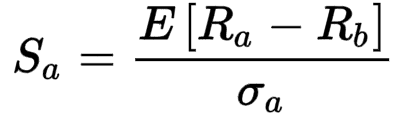
\includegraphics{Sharpe} 
\\
\\
where
\[ R_a = asset\ return \] 
\[ R_b = risk\ free\ return \] 
\[ E = expected\  value \] 
\[ \sigma_a = standard\ deviation\ of\ the\ asset\ excess\ return \] 

The Sharpe ratio tells the expected profit when accounting for loss. A portfolio can earn 100\% profit one month and seem like its an incredibly profitable strategy. However, if it loses 100\% for the next six months, then that means the trading strategy, or in our case the agents policy, is not efficiently profitable, it just happened to get lucky during the first month. Profit is important, but only if the risk is also calculated. We will evaluate the Sharpe ratio that each agent is capable of earning to ensure that the agent profits without risking too much of its assets.
	
\section{6 Timeline}
\begin{center}
\begin{tabular}{||c|c|||} 
 \hline
 Date & Task \\ [0.5ex] 
 \hline\hline
 09/29/2021 & Data Collected and Organized \\ 
 \hline
 10/06/2021 & Envrionment Created \\
 \hline
 10/13/2021 & Q-Learning Training Completed \\
 \hline
 10/16/2021 & Results Evaluated \\
 \hline
 10/18/2021 & Midterm Presentations \\ [1ex] 
 \hline
\end{tabular}
\end{center}

\section{7 Conclusion}
By starting out with a traditional Q-learning method, and graduating to a Deep Q Network learning method, we are certain to see how neural networks can defeat many of the limitations seen by the earlier reinforcement learning methods. Furthermore, we are confident that the DQN learning method will produce a policy that produces greater profit, and a better Sharpe ratio, than most any human controlled portfolio trading under the same circumstances. Lastly, we also plan on finding a less generalized policy compared to the policies learned by agents in other papers because of our methodology of training on many different coin's histories. 

\section{References}
\smallskip \noindent \textit{B. Huang, Y. Huan}\\
Automated trading systems statistical and machine learning methods and hardware implementation: A survey Enterprise Information Systems, L.D. Xu, L. Zheng, Z. Zou 2019. \textit{Blackboard Systems.} 13 (1) (2019), pp. 132-144

\smallskip \noindent \textit{Roderick, M., MacGlashan, J, Tellex, S} 
Implementing the deep Q-network.  Humans To Robots Laboratory, Brown University, Providence, RI 02912, CoRR (2017)

\smallskip \noindent \textit{Mnih, V., Kavukcuoglu, K., Silver, D. et al}\\
Human-level control through deep reinforcement learning. Nature 518, 529–533 (2015). 
https://doi.org/10.1038/nature14236

\smallskip \noindent \textit{Jae Won Lee} 
Stock price prediction using reinforcement learning. ISIE 2001. 2001 IEEE International Symposium on Industrial Electronics Proceedings (Cat. No.01TH8570), 2001, pp. 690-695 vol.1, 
doi: 10.1109/ISIE.2001.931880.

\smallskip \noindent \textit{Yong Shi, Wei Li, Luyao Zhu, Kun Guo, Erik Cambria}
Stock trading rule discovery with double deep Q-network. Applied Soft Computing. Volume 107. 2021. 107320. ISSN 1568-4946.
https://doi.org/10.1016/j.asoc.2021.107320.


\end{document}
